\documentclass[10pt]{article}
\usepackage{icmlko}

\icmlmeta{IP 파운데이션 월드모델}{346}{쟀는데 안 올린 것}{아이돌 넓힘을 열두 노트 전에 재고 기록까지 해 놓고 기본 판에는 안 넣고 있었다}

\begin{document}

\twocolumn[
\icmlheader

\begin{abstract}
노트 325$\sim$334가 아이돌 라벨 기준 필터를 풀어 학습을 54행에서 122행으로
늘리는 것을 재고 \texttt{denominator.json} 에 \textbf{자료 결정으로 기록}까지
했다. \textbf{그런데 기본 축 세트는 여전히 81행을 쓰고 있었다} ---
\texttt{idolwide\_full} 은 팔로만 있고 챔피언이 아니었다.

\textbf{그 사이에 판이 자랐다.} 노트 337이 위키 목록에 아이돌을 넣었고
(덮음 82\%), 노트 333이 검색을 169건 다 긁었고, 노트 343$\sim$345가 태그
축을 넷 늘렸다. \textbf{그래서 다시 쟀다.}

\begin{center}\small
\begin{tabular}{lrr}
\hline
 & 노트 333 & \textbf{오늘} \\
\hline
81행 & 0.2385 & 0.2831 \\
147행 & 0.5115 & \textbf{0.4215} \\
차 & $+$0.2730 & \textbf{$+$0.1384} \\
\hline
\end{tabular}
\end{center}

\textbf{이득이 반으로 줄었다} --- 미리 적은 대로다(``기본 판이 이미 그
이득의 일부를 갖고 있다''). 위키와 검색이 아이돌에 붙으면서 넓힘이 주던
것을 일부 먼저 가져갔다.

\textbf{그래도 크다.} 짝지어 열둘 --- 아이돌 \textbf{$+$0.1587}(SD 0.0694 ·
\textbf{12/12}) · 판 $+$0.0021(SD 0.0057 · 8/12 · 폭 안). 제일 나쁜
도메인이 시장팝업 $-$0.0196($t{\approx}0.5$)이라 배포 규칙 ①② 를 통과한다.
\textbf{챔피언 축 세트를 \texttt{idolwide\_full} 로 올린다.}

\textbf{왜 열두 노트가 걸렸나.} 자료 결정을 \emph{기록}하는 것과 기본
경로를 \emph{바꾸는} 것이 이 판에서는 다른 일이다 --- 축 세트가 팔로
존재하면 잰 것으로 끝나고, 아무도 그것을 기본으로 만들지 않는다.
\textbf{``쟀다''와 ``쓴다''는 다르다.}
\end{abstract}
]

\section{기록은 했는데 안 썼다}

\begin{center}\footnotesize
\begin{tabular}{ll}
\hline
노트 326 & 막은 것이 라벨이 아니라 수집 경로다 \\
327 & 넣으면 $+$0.088 · 위약 대비 $p{=}0.033$ \\
332 & 위키를 긁어 그림자를 지웠다 \\
333 & 앨범 필터도 떼고 검색을 다 긁었다 \\
334 & 배포는 ``앨범 축 둘 뺀 채'' \\
\textbf{그리고} & \texttt{denominator.json} 에 자료 결정으로 기록 \\
\hline
\textbf{그런데} & \textbf{기본 축 세트는 81행 그대로} \\
\hline
\end{tabular}
\end{center}

\begin{figure*}[t]
\centering
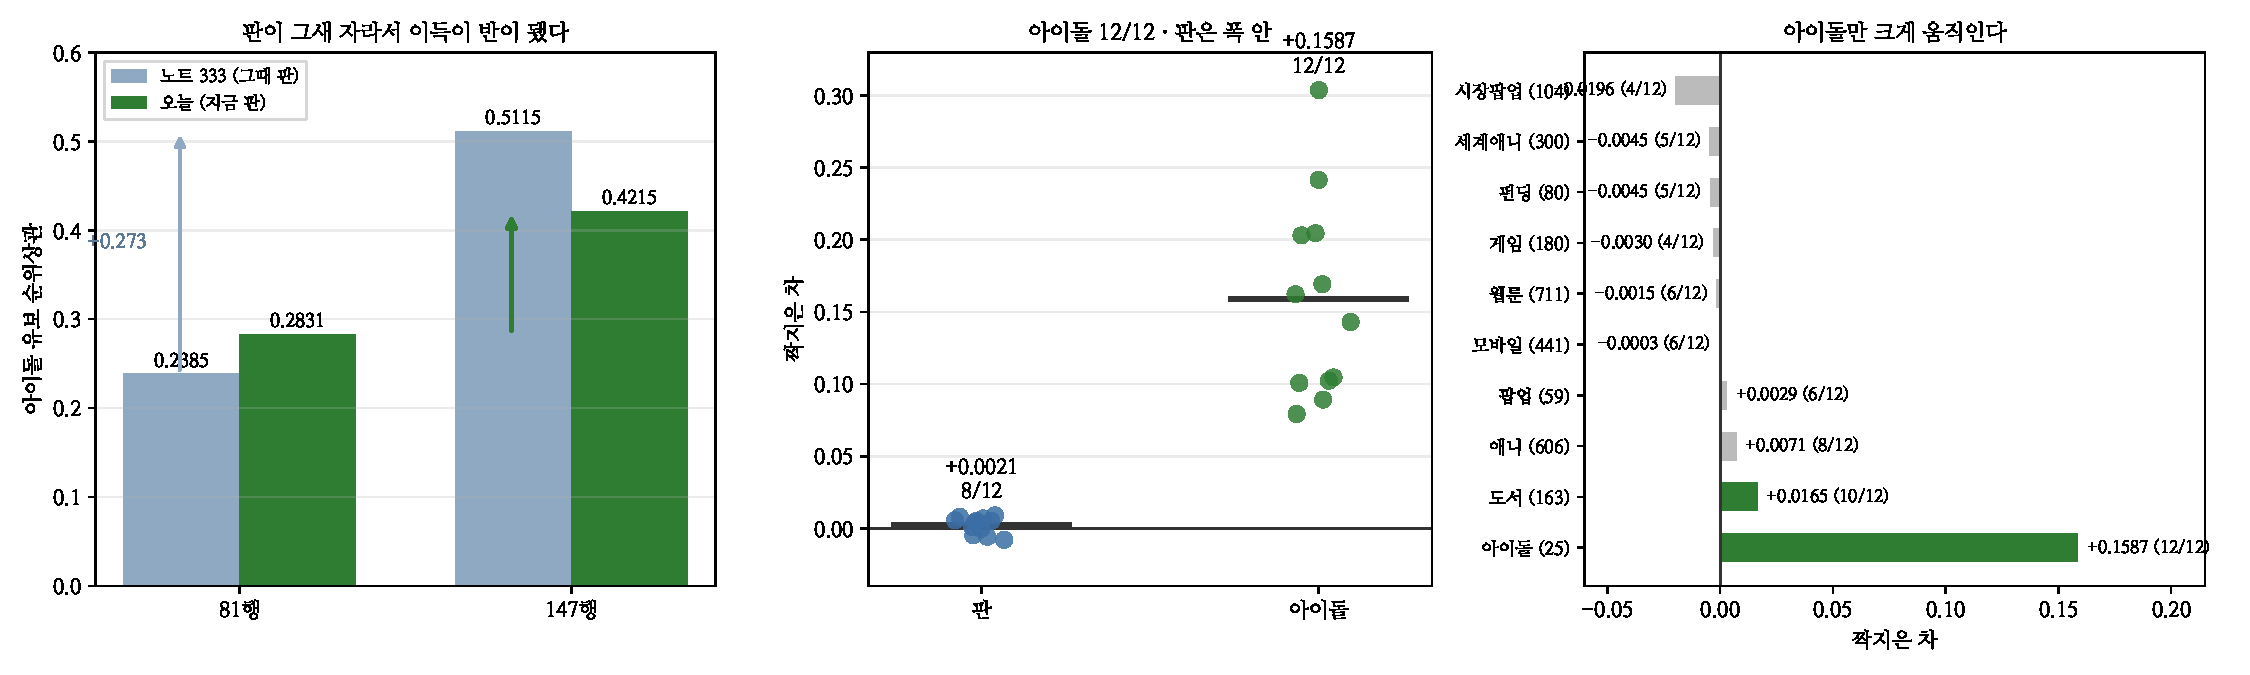
\includegraphics[width=\textwidth]{figs/promote.pdf}
\caption{왼쪽 --- 노트 333과 오늘. 가운데 --- 짝지은 차.
오른쪽 --- 도메인별.}
\end{figure*}

\section{판이 자라서 이득이 반이 됐다}

\begin{center}\footnotesize
\begin{tabular}{ll}
\hline
그 사이에 바뀐 것 & \\
\hline
노트 337 & \texttt{wikiaxes.AXF} 에 아이돌 --- 덮음 82\% \\
노트 333 & 검색 44 $\to$ 169건 \\
노트 343$\sim$345 & 태그 축 넷 추가 \\
\hline
\end{tabular}
\end{center}

\textbf{81행 쪽이 0.2385 에서 0.2831 로 올라왔다.} 넓힘이 주던 것 중
위키 · 검색이 줄 수 있는 몫을 기본 판이 먼저 가져간 것이다.
\textbf{미리 적은 실패가 맞았다.}

\section{그래도 붙인다}

\begin{center}\footnotesize
\begin{tabular}{lrrr}
\hline
 & 평균 & SD & 양수 \\
\hline
\textbf{아이돌} & \textbf{$+$0.1587} & 0.0694 & \textbf{12/12} \\
도서 & $+$0.0165 & 0.0284 & 10/12 \\
애니 & $+$0.0071 & 0.0116 & 8/12 \\
시장팝업 & $-$0.0196 & 0.0628 & 4/12 \\
세계애니 & $-$0.0045 & 0.0083 & 5/12 \\
\hline
판 & $+$0.0021 & 0.0057 & 8/12 \\
\hline
\end{tabular}
\end{center}

배포 규칙 ①(판 폭 안) ②(제일 나쁜 시장팝업 $-$0.0196 · 짝SE 0.04 ·
$t{\approx}0.5$)를 통과한다. \textbf{그리고 이것은 축이 아니라 자료
결정이다}(노트 82 · 90) --- 라벨 필터를 뗀 것과 수집기를 고친 것뿐이고
점수로 고른 것이 아니다.

\paragraph{유보는 그대로} 147행은 학습만 늘린 것이다 --- 추가 94건 중
2025년 이후 26건은 버렸다. \textbf{판 분모가 2,675 그대로}라 옛 점수와
직접 견줄 수 있다.

\section{남은 것}
\begin{center}\footnotesize
\begin{tabular}{ll}
\hline
갈래 & 왜 \\
\hline
\textbf{버린 26행} & 유보를 25 $\to$ 51 로 --- 과제가 바뀐다 \\
시장팝업이 왜 또 지나 & 노트 342 · 345 에서도 \\
다른 ``쟀는데 안 쓴 것'' & 이번이 처음이 아닐 것 \\
앨범 축 둘 & 노트 334 이후 안 다시 봤다 \\
\hline
\end{tabular}
\end{center}

\paragraph{규약} \textbf{``쟀다''와 ``쓴다''는 다르다.} 이 실험실은 축 세트를
팔로 만들어 견주는데, 이기고 나서 \emph{기본이 되는} 절차가 없다 ---
\texttt{denominator.json} 에 적는 것은 기록이지 배선이 아니다. 그래서
아이돌 넓힘이 열두 노트 동안 ``이미 한 일''로 취급되면서 실제로는 안
돌고 있었다. \textbf{이 판에서 갈라진 목록을 여섯 번 찾았는데, 이번 것은
목록이 아니라 \emph{내 기억}이 갈라진 것이다.} 자료 결정을 적을 때
\textbf{``어느 축 세트가 그것을 쓰나''}를 같이 적어야 한다.

\end{document}
